\documentclass[class=bu430,notes,tikz]{agony}
\usetikzlibrary{fit}
\declaretheorem[Refname={Game,Games},refname={game,games},style=thmroundred,sibling=theorem]{game}

\title{BU 430 Spring 2025: Lecture Notes}

\begin{document}
\renewcommand{\contentsname}{BU 430 Spring 2025:\\{\huge Lecture Notes}}
\thispagestyle{firstpage}
\tableofcontents

Lecture notes taken, unless otherwise specified,
by myself during section J of the Spring 2025 offering of BU 430,
taught by Michael Brolly.

\begin{multicols}{2}
  \listoflecture
\end{multicols}

\chapter{Introduction}

\lecture{May 5}
In general, previous finance courses have considered
\[ \text{return} = \text{opportunity cost} + \text{risk premium} + \text{transaction costs} \]
where we have only cared about the opportunity cost (risk-free rate)
and risk premium.

This leads to treating the market as a zero-sum game
where if A sells a share of \vv{XYZ} to B for \$10,
then A gains \$10 cash, B gains \$10 value, and the total is a wash.

In reality, the market is a negative-sum game:
A sells for \$9.90 to a market maker and B buys for \$10.10 from the market maker,
so the total is $-20$\textcent.

Why are transaction costs necessary?
A perfect market should have liquidity (investors can cheaply trade as much and as often as they want)
and price efficiency (the asset value should be reflected quickly and accurately).
In reality, investors don't arrive continuously throughout the day,
provide a naturally balanced book, or reveal information freely.


\chapter{The market landscape}
\lecture{May 7}


\section{Limit markets}

\section{The order book}
\lecture{May 12}

\section{Trading on margin}
\lecture{May 14}

\begin{defn}[margin ratio]
  The margin ratio is given by
  \[ \frac{\text{equity value}}{\text{market value of assets}} = \frac{\text{market value of assets} - \text{loan}}{\text{market value of assets}} \]
  At the moment of investment, the margin ratio is
  \[ \frac{P \times Q - \text{loan}}{P \times Q} \]
  and at some later time,
  \[ \frac{(P + \text{dividends})\times Q - \text{loan}}{(P + \text{dividends}) \times Q} \]
\end{defn}

\begin{example}
  Suppose an investor has \$10,000 in cash.
  They wish to buy 1,000 shares of stock at \$20 per share.
  What is their initial margin ratio?
\end{example}
\begin{sol}
  \[ \text{margin ratio} = \frac{\text{investor equity}}{P \times Q} = \frac{10000}{1000 \times 20} = 0.5 \qedhere \]
\end{sol}

\begin{example}
  Suppose the price of the stock drops from \$20 per share to \$15 per share.
  What is the investor's new margin ratio?
\end{example}
\begin{sol}
  First find the loan amount $(P \times Q) - \text{equity} = 1000 \times 20 - 10000 = 10000$. Then,
  \[ \frac{(P + \text{dividends})\times Q - \text{loan}}{(P + \text{dividends}) \times Q} = \frac{15 \times 1000 - 10000}{15 \times 1000} = \frac13 \qedhere \]
\end{sol}

The bearish equivalent of going long on margin is to \term[short selling]{short sell},
where the seller borrows a stock, sells it, and then buys it back later.
If the seller does not first borrow a stock, it is a \term[short selling!naked]{naked short},
which is largely illegal now.

\lecture{May 19}
\section{Settlement and clearing}

\lecture{May 21}

\section{Market rules}
\lecture{May 26}
The stock market has fragmented in recent years,
so how do investors know what the best price across all markets is?

\begin{defn*}[order protection rule]
  The \term{Canada Protected Bid Offer} (CPBO) and \term{National Best Bid Offer} (NBBO)
  are the best bid/ask prices and volume from all \term[protected venue]{protected venues}.
  A venue is awarded protection by regulators.

  The \term{order protection rule} (OPR) requires that brokers send orders
  to the protected venues displaying the CPBO/NBBO.
  The broker can only route to an unprotected venue if the price is strictly better.
\end{defn*}

\begin{example}
  Suppose the NBBO for \vv{XYZ} is a bid for 300 @ 49.95 on exchange A
  to an ask for 100 @ 50.00 on exchange B.

  If a new ask for 300 @ 49.99 arrives to exchange A, the new NBBO is 49.95/49.99.

  If another new ask for 200 @ 49.97 arrives to unprotected exchange C,
  the NBBO is unchanged at 49.95/49.99.

  If
\end{example}

In Canada, the protected venues are the NEO-L, TSX, TSXV, CSE, Nasdaq CXC,
Nasdaq CX2, and Omega ETS exchanges.

\lecture{May 28}
What happens if many limit orders are at the NBBO?
Typically, price ties are broken by time of arrival.

\section{Advanced order types}

Some fancy order types exist for precision timing:
\begin{defn}
  An \term[order!immediate-or-cancel]{immediate-or-cancel} (IOC) order
  fills what it can in the moment and cancels any unfilled portion.

  A \term[order!fill-or-kill]{fill-or-kill} (FOK) order requires
  the entire order to be filled immediately, otherwise the entire order is cancelled.

  A \term[order!market-on-close]{market-on-close} (MOC) order
  triggers at the end of the trading day.
\end{defn}
IOC and FOK orders don't leave signals for others to pick up on your intention
and can avoid adverse market conditions.
HFTs use FOK orders to ``ping'' for hidden liquidity.

MOC orders are useful to implement strategies that rely on closing prices.

Consider the order book:
\begin{center}
  \begin{tabular}{cc||cc}
    Bid   & Quantity & Ask   & Quantity \\ \hline
    49.75 & 500      & 50.25 & 100      \\
    49.50 & 800      & 51.50 & 200      \\
    49.25 & 500      & 54.75 & 300      \\
    49.00 & 200      & 58.25 & 100
  \end{tabular}
\end{center}
If a trader submits an IOC buy order for 200 @ 50.50,
the first 100 shares get taken at 50.25 and the remaining 100 are cancelled.

If a trader submits a FOK buy order for 200 @ 50.50, nothing would happen at all.

Other order types exist to automate the exiting of a position.

\begin{defn}
  A \term[order!stop]{stop} (STOP) order triggers a sell (resp.\ buy)
  market order when the price moves below (resp.\ above) a certain limit price.

  A \term[order!stop limit]{stop limit} order (SLO) triggers a sell (resp.\ buy)
  limit order when the price moves below (resp.\ above) a certain limit price.
\end{defn}

These manage risk for traders not constantly watching the market
and can avoid slippage from sharp movements like flash crashes.

\begin{defn}
  All orders are either \term[order!good-till-day]{good-till-day} (GTD),
  where they expire at the end of the trading day,
  or \term[order!good-till-cancelled]{good-till-cancelled} (GTC),
  where they are re-entered daily until filled.
\end{defn}

Other fun order types exist (dark orders, pegged orders) that will be covered later.

\section{Measuring liquidity}
\lecture{June 2}

The best measure of liquidity in the market is the bid--ask spread:

\begin{defn}
  Suppose we are in a limit market with ask price $a$, bid price $b$,
  and midpoint $\frac12(a+b)$.
  The \term[spread!absolute]{absolute} (or \term[spread!quoted]{quoted}) \term*{spread}
  is given by
  \[ S := a - b \]
  The \term[spread!relative]{relative spread} (or \term[spread!percentage]{percentage quoted spread}) is
  \[ s := \frac{S}{m} = \frac{a-b}{\frac12(a+b)} \]
\end{defn}

\begin{example}
  BCE has a quoted bid of \$43.35 and an ask of \$44.20.
  What is the (absolute) quoted spread $S$ in dollars and percentage terms?
\end{example}
\begin{sol}
  In dollar terms: $S = \$44.20 - \$43.55 = \$0.85$.

    In percentage terms: $s = \frac{\$0.85}{\frac12(\$44.20+\$43.35)} = 1.94\%$.
\end{sol}

\begin{example}
  If \vv{BCE} has a relative spread of 1.94\% (on quotes of bid/ask 43.35/44.20),
  and \vv{RCI} has a quoted bid of \$38.25 and an ask of \$38.63, which stock is
  ``more liquid''?
\end{example}
\begin{sol}
  Find $s_{\vv{RCI}} = \frac{a-b}{m} = \frac{38.63-38.25}{0.5(38.63+38.25)} = 0.99\%$.

  Since $0.99\% < 1.94\%$, RCI is more liquid.
\end{sol}

If we perform a transaction, we are not guaranteed to execute at the bid/ask.
Therefore, the spread we experience is not $S$.

\begin{defn}
  Suppose the market has a midpoint $m$, and we execute at $p$.
  Then, the \term[spread!effective, half-]{effective half-spread} is
  \[ S_e := \abs{p - m} = d(p - m) \]
  where the direction $d = 1$ for buys and $-1$ for sells.
\end{defn}

This is a retrospective analysis of a past trade,
whereas the ordinary quoted spread is prospective for a hypothetical trade.

If the entire order did not execute at $p$,
we use the \term[price!volume-weighted average]{volume-weighted average price}
$\frac{1}{V}\sum_{p_i} V_i p_i$.

Although the effective spread is the cost to trade,
market makers are not guaranteed to profit by $S_e$.
To offload the position at time $t+\Delta$, they experience another spread,
the \term[spread!realized, half-]{realized half-spread}:
\[ S_r := d_t(p_t - m_{t+\Delta}) = \underbrace{d_t(p_t - m_t)}_{\mathclap{\text{effective half-spread}}} - \underbrace{d_t(m_{t+\Delta} - m_t)}_{\text{price impact}} \]
Some people use VWAP-based spread as a metric for brokers, but this is gameable:
after a large price movement, VWAP decouples from the spot price.
Therefore, VWAP-benchmarking incentivizes trades early in the day,
even if prices have moved favourably for the client.

In general, when a buy (resp.\ sell) order hits the market, it tends to
increase (resp.\ decrease) the midpoint.
\begin{lemma}
  The \term{price impact} on the midpoint at time $t$ can be expressed as
  \[ \Delta m_t = \lambda x_t + \varepsilon_t \]
  linear in the order imbalance $x_t$ between $t-1$ and $t$
  with price impact coefficient $\lambda \approx \frac{1}{\text{depth}}$.
  The transitive impact $\varepsilon_t$ is noisy,
  and we just hope it gets cancelled out by future noise.
\end{lemma}

The absolute change in prices $\abs{\Delta m_t}$ is correlated with trading volume $V_t$.
\begin{defn}
  The \term{order imbalance} $x_t$ is the difference between the number of shares
  traded in buyer-initiated transactions (positive)
  and seller-initiated transactions (negative).

  The \term{Amihud illiquidity ratio} is given by
  \[ I_t := \frac{\abs{\Delta m_t}}{\abs{x_t}} \]
  or equivalently the Amihud liquidity ratio $L_i := \frac{1}{I_t}$
\end{defn}

\begin{lemma}
  We can approximate order imbalance $\abs{x_t}$ with price volume $p_t V_t$
  and open/close midpoints with open/close prices, so that
  \[ I_t \approx \frac{\abs{p_t-p_{t+1}}}{p_tV_t} = \frac{\abs{r_t}}{V_t} \]
  with the rate of return $r_t = \frac{p_t - p_{t+1}}{p_t}$.
\end{lemma}

\begin{example}
  Consider two telecom stocks, \vv{BCE} and \vv{RCI}\@.
  From May 20 to May 21, \vv{BCE} went from (close-to-close),
  30.15 to 29.79 on a volume of 4,405,500; \vv{RCI} went from
  35.88 to 36.09 on a volume of 1,737,900. According to the Amihud illiquidity
  measure, which stock was more liquid that day?
\end{example}
\begin{sol}
  Calculate:
  \begin{align*}
    I_t^{\vv{BCE}} & = \frac{\abs{\frac{29.79-30.15}{30.15}}}{4405500} = 2.79\times 10^{-9} &
    I_t^{\vv{RCI}} & = \frac{\abs{\frac{36.09-35.88}{35.88}}}{1737900} = 3.37\times 10^{-9}
  \end{align*}
  Since $I_t^{\vv{RCI}} > I_t^{\vv{BCE}}$, \vv{RCI} was more illiquid, i.e.,
  \vv{BCE} was more liquid.
\end{sol}

Instead of VWAP, how can we measure a broker's efficiency?
Suppose there was a perfect market which \emph{could} trade the client's
entire (signed) order $q$ at the midpoint.
Then, after time $t$, that ``paper portfolio'' would have return
\[ R_p = q(m_t - m_0) \]
If in reality the broker only got a fraction $\kappa$ of the order
executed at average price $\bar p$, the client experiences return
\[ R_a = \kappa q(m_t - \bar p) \]
We can measure the difference.

\begin{defn}
  The \term{implementation shortfall} is
  \[ IS := R_p - R_a = q(m_t - m_0) - \kappa q(m_t - \bar p) \]
\end{defn}

We can divide the implementation shortfall into two components:
\begin{align*}
  IS & = q(m_t - m_0) - \kappa q(m_t - \bar p)                                                                                         \\
     & = \underbrace{\kappa q(\bar p - m_0)}_{\text{execution cost}} + \underbrace{(1-\kappa) q (m_t - m_0)}_{\text{opportunity cost}}
\end{align*}
since \emph{not trading} has the cost of not experiencing the return.
Because opportunity cost is measured, this can't be gamed in the same way as VWAP.

\begin{example}
  Suppose I wanted to buy 10,000 shares when $m_0 = 100$.
  Later, the broker actually executes 3,000 shares at $\bar p = 101$.
  Now, the price is 103.
  How are they doing?
\end{example}
\begin{sol}
  Calculate $(3,000 \cdot (101 - 100)) + (7,000\cdot (103-100)) = 3,000 + 21,000 = 24,000$.

  This shortfall is $\frac{24,000}{m_0 q} = 2.4\%$ of a perfect portfolio.
\end{sol}

\lecture{June 4}
In general, $IS$ is computed by averaging over many trades, i.e.,
\[ \E[IS] = \kappa\E[q(\bar p - m_0)] + (1-\kappa)\E[q\Delta m] \]
Reducing $\E[q(\bar p-m_0)]$ can be done with more patient trading,
but this has a trade-off with opportunity cost.

The $\E[q\Delta m]$ term can be positive because the client is trading
on the same information as others in the market or because of front-running.

\chapter{Game theory}

\section{Symmetric games}

\begin{defn}
  A \term{game} generally consists of players, actions, and payoffs.

  A \term[game!simultaneous]{simultaneous game} has all players act at once
  (i.e., no time advantage).

  A \term[game!symmetric]{symmetric game} means all players
  have access to the same information.
\end{defn}

The prisoner's dilemma is a classic example of a simultaneous symmetric game.

\begin{game}[prisoner's dilemma]\label{g:pd}
  A and B have been arrested and are being interrogated separately.
  If both cooperate they serve 1 year.
  If one flips, the betrayer goes free and the other serves 3 years.
  If both flip, they serve 2 years.
  \begin{center}
    \begin{tabular}{cc|c|cc}
       & \multicolumn{3}{c}{\footnotesize B}                      \\
      \multirow{3}{*}{\rotatebox[origin=c]{90}{\footnotesize A}}
       &                                     & Cooperate & Betray \\ \cline{2-4}
       & Cooperate                           & (1,1)     & (3,0)  \\ \cline{2-4}
       & Betray                              & (0,3)     & (2,2)
    \end{tabular}
  \end{center}
\end{game}

\begin{defn}
  A \term{Nash equilibrium} is a set of strategies for all players where,
  given the strategies of other players,
  no player can improve their payoff by altering their strategy.
\end{defn}

In \cref{g:pd}, the Nash equilibrium is for both to flip,
since $0 < 1$ (if other cooperates) and $2 < 3$ (if other flips).

\begin{game}[matching pennies]
  Two players hold a penny in their hand either heads or tails.
  Player 1 wins if they choose the same side and Player 2 wins if they choose different.
  \begin{center}
    \begin{tabular}{cc|C|CC}
       & \multicolumn{3}{c}{\footnotesize Player 2}                   \\
      \multirow{3}{*}{\rotatebox[origin=c]{90}{\footnotesize Player 1}}
       &                                            & H      & T      \\ \cline{2-4}
       & $H$                                        & (1,-1) & (-1,1) \\ \cline{2-4}
       & $T$                                        & (-1,1) & (1,-1)
    \end{tabular}
  \end{center}
\end{game}
There is no pure strategy Nash equilibrium since there is no preference.

Instead, players can choose stochastic strategies such that
all actions in their strategy have equal payoffs given the strategies of others.
That is, for all Player 1 actions $a_1 \neq a_1'$ and Player 2 strategies $s_2$,
$\pi_1(a_1 \mid s_2) = \pi_1(a_1' \mid s_2)$.

Suppose Player 2 picks heads with probability $p_2$.
If $p_2 < 0.5$, Player 1 should always choose tails $p_1(p_2) = 0$.
If $p_2 > 0.5$, Player 1 should always choose heads $p_1(p_2) = 1$.
Graphically:
\begin{center}
  \begin{tikzpicture}
    \begin{axis}[
        xlabel={$p_1$},
        ylabel={$p_2$},
      ]
      \addplot[blue, thick, domain=0:0.5] {0};
      \addplot[blue, thick, domain=0.5:1] {1};
      \addplot[blue, thick] coordinates {(0.5, 0) (0.5, 1)};
    \end{axis}
  \end{tikzpicture}
\end{center}
The same logic applies to Player 2 choosing a strategy:\footnote{``I'm not suggesting that this is the worst thing that came out of World War II, but this is really annoying''}
\begin{center}
  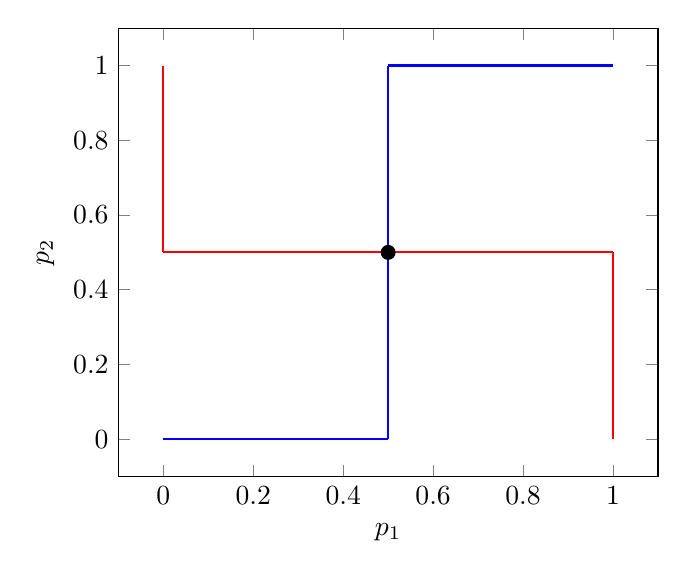
\begin{tikzpicture}
    \begin{axis}[
        xlabel={$p_1$},
        ylabel={$p_2$},
      ]
      \addplot[blue, thick, domain=0:0.5] {0};
      \addplot[blue, thick, domain=0.5:1] {1};
      \addplot[blue, thick] coordinates {(0.5, 0) (0.5, 1)};
      \addplot[red, thick, domain=0:1] {0.5};
      \addplot[red, thick] coordinates {(0, 1) (0, 0.5)};
      \addplot[red, thick] coordinates {(1, 0.5) (1, 0)};
      \addplot[only marks, mark=*, mark size=2.5pt, black] coordinates {(0.5, 0.5)};
    \end{axis}
  \end{tikzpicture}
\end{center}
The equilibrium is for both players to flip with $\frac12$ probability.

\begin{game}[battle of the sexes]
  Harry and Sally are deciding where to meet.
  \begin{center}
    \begin{tabular}{cc|c|cc}
       & \multicolumn{3}{c}{\footnotesize Harry}                     \\
      \multirow{3}{*}{\rotatebox[origin=c]{90}{\footnotesize Sally}}
       &                                         & Local & Starbucks \\ \cline{2-4}
       & Local                                   & 1,2   & 0,0       \\ \cline{2-4}
       & Starbucks                               & 0,0   & 2,1
    \end{tabular}
  \end{center}
\end{game}
This (both players want equality) is similar to
the matching pennies game (only one wants equality).
There are two Nash equilibria: $(1,2)$ and $(2,1)$.

Suppose the game is not simultaneous,
and Sally starts by proposing a coffee spot $a_S$.
Then, Harry will always follow Sally to $a_S$.
But knowing that Harry will do this, Sally always chooses Starbucks.

This is a \term[Nash equilibrium!subgame perfect]{subgame perfect Nash equilibrium} (SPNE).

SPNEs can rule out nonsense equilibria.
\begin{game}[new entrants]
  An incumbent is deciding how to treat a potential new entrant:
  \begin{center}
    \begin{tabular}{cc|c|cc}
       & \multicolumn{3}{c}{\footnotesize Incumbent}                         \\
      \multirow{3}{*}{\rotatebox[origin=c]{90}{\footnotesize Entrant}}
       &                                             & Fight   & Accommodate \\ \cline{2-4}
       & Out                                         & 0,2     & 0,2         \\ \cline{2-4}
       & In                                          & $-3,-1$ & 2,1
    \end{tabular}
  \end{center}
\end{game}
Technically, this implies there are two Nash equilibria:
(no entry, price war) and (entry, accommodation).
There's no way to price war if there's no entry, so this makes no sense.
We can picture this graphically:
\begin{center}
  \begin{tikzpicture}
    \graph[layered layout, grow down, sibling distance=2cm, level distance=1.4cm] {
      Entrant -- {
      "0,2"[>"Out" above left],
      Incumbent[>"In"] -- {"$-3,-1$"[>"Fight" above left], "2,1"[>"Accommodate"]}};
      };
  \end{tikzpicture}
\end{center}
and then build from the bottom-up (backward induction).

\section{Bayesian games}
\lecture{June 9}

What happens if one person knows more than the other.
For example, a trader knows why they are trading, but a market maker does not.
Consider a more complicated version of the last game:
\begin{game}[Bayesian new entrants]\label{g:ne}
  An incumbent is deciding how to treat a potential new entrant:
  \begin{center}
    \begin{tikzpicture}[node quotes mean={label={[#2,font=\small]#1}}]
      \graph[layered layout, sibling distance=2cm, level distance=1.4cm] {
        "Nature of Entrant" -- {
        "Out (0.25)" -- "0,2",
        "Aggressive (0.5)" -- A/Incumbent-- {"$-5,-4$"[>"Fight" left], "$3,-7$"[>"Acc."]},
        "Passive (0.25)" -- P/Incumbent -- {"$-3,-1$"[>"Fight" left], "2,1"[>"Acc."]}
        };
        };
        \node[draw,dotted,fit=(A) (P)] {};
    \end{tikzpicture}
  \end{center}
  where the dashed box indicates that the Incumbent cannot distinguish
  between the two states.
\end{game}
We call sequential asymmetric information games like this \term[game!Bayesian]{Bayesian games}.

\begin{prop}[probability basics]
  Recall:
  \begin{itemize}
    \item $\Pr[A^\complement] = 1-\Pr[A]$
    \item $\Pr[A \cup B] = \Pr[A] + \Pr[B] + \Pr[A \cap B]$
    \item $\Pr[A \cap B] = \Pr[A] \cdot \Pr[B]$ if $A$ and $B$ are independent
    \item $\Pr[A \mid B] = \frac{\Pr[A \cap B]}{\Pr[B]}$
  \end{itemize}
\end{prop}
\begin{theorem}[Bayes' rule]\label{thm:bayes}
  \[ \Pr[A \mid B] \Pr[B] = \Pr[B \mid A] \Pr[A] \]
  or equivalently
  \[ \Pr[A \mid B] = \frac{\Pr[B \mid A]\Pr[A]}{\Pr[B]} = \frac{\Pr[B \mid A]\Pr[A]}{\Pr[B \mid A]\Pr[A] + \Pr[B\mid A^\complement]\Pr[A^\complement]} \]
\end{theorem}

\begin{example}
  The bank knows that
  \begin{itemize}[nosep]
    \item 5\% of borrowers default;
    \item 95\% of borrowers do not default;
    \item Of defaults, 70\% had low credit scores; and
    \item Of non-defaults, 20\% had low credit scores.
  \end{itemize}
  How likely is it for a low-score borrower to default?
\end{example}
\begin{sol}
  Apply \nameref{thm:bayes}:
  \begin{align*}
    \Pr[D \mid L]
     & = \frac{\Pr[L \mid D]}{\Pr[L \mid D]\Pr[D] + \Pr[L \mid D^\complement]\Pr[D^\complement]} \\
     & = \frac{0.7}{0.7\cdot 0.05 + 0.2\cdot 0.95}                                               \\
     & \approx 0.1556
  \end{align*}
  So the probability is about 15.56\%.
\end{sol}

Now, consider again \cref{g:ne}.
When the Incumbent gets to play, we are given that the Entrant entered.
We can read off that $\Pr[Agg \mid In] = \frac23$ and $\Pr[Pass \mid In] = \frac13$.
So the expected value of playing Fight $F$ is
\begin{align*}
  \E[\pi_{Inc} \mid F]
   & = \Pr[Agg \mid In] \cdot \pi_{Inc}(F \mid Agg) + \Pr[Pass \mid In]\cdot \pi_{Inc}(F \mid Agg) \\
   & = \frac23(-4) + \frac13(-1) = -3
\end{align*}
and the expected value of playing Accommodate $A$ is
\begin{align*}
  \E[\pi_{Inc} \mid A]
   & = \Pr[Agg \mid In] \cdot \pi_{Inc}(A \mid Agg) + \Pr[Pass \mid In]\cdot \pi_{Inc}(A \mid Agg) \\
   & = \frac23(-8) + \frac13(1) = -5
\end{align*}
so the Incumbent will prefer to fight.

\begin{game}[the market for lemons]
  Suppose there are equal shares good cars and bad cars on the used car market.
  Good cars are valued by sellers at \$10k and buyers at \$15k.
  Bad cars are valued by sellers at \$8k and buyers at \$12k.
  The sellers know if a car is bad, but buyers do not.

  What price do sellers sell at?
\end{game}

The expected value of a car to the buyers is \$13.5k,
so sellers will price there.
This results in a profit for the seller in either case.
A seller of a good car cannot offer a higher price since there is no way to prove
that it is a good car.

Suppose instead that good cars are valued by sellers at \$12k and buyers at \$15k.
Bad cars are valued by sellers at \$6k and buyers at \$8k.

Buyers now value cars at \$11.5k each given that there is a 50\% chance of a good car.
But selling good cars would have negative value,
so sellers are only willing to sell bad cars.
However, buyers know this and will only buy for the lower bad car equilibrium price of \$8k.

In this case, good cars exist but will never be sold.

\pagebreak
\phantomsection\addcontentsline{toc}{chapter}{Back Matter}
% \renewcommand{\listtheoremname}{List of Named Results}
% \phantomsection\addcontentsline{toc}{section}{\listtheoremname}
% \listoftheorems[ignoreall,numwidth=4em,onlynamed={theorem,lemma,corollary,prop}]
\printindex

\end{document}
